% $Id: template.tex 11 2007-04-03 22:25:53Z jpeltier $
\newcommand{\todo}[1]{{\bf \{TODO: {#1}\}}}
\newcommand{\projectname}{Story Explorer}

\documentclass{vgtc}                          % final (conference style)
%\documentclass[review]{vgtc}                 % review
%\documentclass[widereview]{vgtc}             % wide-spaced review
%\documentclass[preprint]{vgtc}               % preprint
%\documentclass[electronic]{vgtc}             % electronic version

%% Uncomment one of the lines above depending on where your paper is
%% in the conference process. ``review'' and ``widereview'' are for review
%% submission, ``preprint'' is for pre-publication, and the final version
%% doesn't use a specific qualifier. Further, ``electronic'' includes
%% hyperreferences for more convenient online viewing.

%% Please use one of the ``review'' options in combination with the
%% assigned online id (see below) ONLY if your paper uses a double blind
%% review process. Some conferences, like IEEE Vis and InfoVis, have NOT
%% in the past.

%% Figures should be in CMYK or Grey scale format, otherwise, colour 
%% shifting may occur during the printing process.

%% These three lines bring in essential packages: ``mathptmx'' for Type 1 
%% typefaces, ``graphicx'' for inclusion of EPS figures. and ``times''
%% for proper handling of the times font family.

\usepackage{mathptmx}
\usepackage{graphicx}
\usepackage{times}

%% We encourage the use of mathptmx for consistent usage of times font
%% throughout the proceedings. However, if you encounter conflicts
%% with other math-related packages, you may want to disable it.

%% If you are submitting a paper to a conference for review with a double
%% blind reviewing process, please replace the value ``0'' below with your
%% OnlineID. Otherwise, you may safely leave it at ``0''.
\onlineid{0}

%% declare the category of your paper, only shown in review mode
\vgtccategory{Research}

%% allow for this line if you want the electronic option to work properly
\vgtcinsertpkg

%% In preprint mode you may define your own headline.
%\preprinttext{To appear in an IEEE VGTC sponsored conference.}

%% Paper title.

\title{\projectname: A Visual Analysis Tool for Heterogeneous Text Data}

%% This is how authors are specified in the conference style

%% Author and Affiliation (single author).
%%\author{Roy G. Biv\thanks{e-mail: roy.g.biv@aol.com}}
%%\affiliation{\scriptsize Allied Widgets Research}

%% Author and Affiliation (multiple authors with single affiliations).
\author{Chenglong Wang%
\and Zhengjie Miao %
\and Siming Chen
\and Zipeng Liu
\and Zuchao Wang
\and Zhenhuang Wang
\and Xiaoru Yuan\thanks{e-mail: \{chenglongwang, miaozhengjie, csm, zipeng.liu, zuchao.wang, wangzhenhuang, xiaoru.yuan\}@pku.edu.cn}}
\affiliation{\scriptsize Peking University}

%% Author and Affiliation (multiple authors with multiple affiliations)
%\author{Chenglong Wang\thanks{e-mail: roy.g.biv@aol.com}\\ %
%        \scriptsize Starbucks Research %
%\and Zhengjie Miao\thanks{e-mail:ed.grimley@aol.com}\\ %
%     \scriptsize Grimley Widgets, Inc. %
%\and Martha Stewart\thanks{e-mail:martha.stewart@marthastewart.com}\\ %
%     \parbox{1.4in}{\scriptsize \centering Martha Stewart Enterprises \\ Microsoft Research}}

%% A teaser figure can be included as follows, but is not recommended since
%% the space is now taken up by a full width abstract.
%\teaser{
%  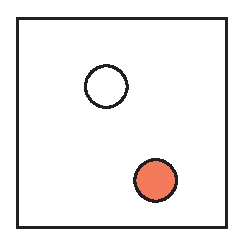
\includegraphics[width=1.5in]{sample.eps}
%  \caption{Lookit! Lookit!}
%}

%% Abstract section.
\abstract{
In this poster, we propose \projectname\ , a visual analytic system for text data from multiple sources. With various visualizations, our system can help analysts identify conflicts and correlations in large volume of text data, and detect patterns of group of people. Thus analysts can discover the development of events and find the suspicious people in the events.
} % end of abstract

%% ACM Computing Classification System (CCS). 
%% See <http://www.acm.org/class/1998/> for details.
%% The ``\CCScat'' command takes four arguments.

%% Copyright space is enabled by default as required by guidelines.
%% It is disabled by the 'review' option or via the following command:
% \nocopyrightspace

%%%%%%%%%%%%%%%%%%%%%%%%%%%%%%%%%%%%%%%%%%%%%%%%%%%%%%%%%%%%%%%%
%%%%%%%%%%%%%%%%%%%%%% START OF THE PAPER %%%%%%%%%%%%%%%%%%%%%%
%%%%%%%%%%%%%%%%%%%%%%%%%%%%%%%%%%%%%%%%%%%%%%%%%%%%%%%%%%%%%%%%%

\begin{document}

%% The ``\maketitle'' command must be the first command after the
%% ``\begin{document}'' command. It prepares and prints the title block.

%% the only exception to this rule is the \firstsection command
\firstsection{Introduction}

\maketitle

Exploring heterogeneous text data from different sources can be complicated and misleading if not well dealing with hidden relationship between entities or possible data conflicts between materials. 
To reveal potential relationship between POK and GAStech in MC1, we need to investigate important information using files from different sources, e.g. employee resumes, email headers, research reports, and a huge volume of news. To solve these challenges, we integrate different kinds of source files into our timeline-based analysis tool \projectname. It serves as a quick overview tool for original data, allowing users to focus only on important files for efficiency. 
\par
In this paper, we will first introduce design challenges of visual analysis tools for heterogeneous text data and how we design \projectname to solve them. Then we will introduce how we use \projectname\ to solve MC1 problems.
%% \section{Introduction} 

%eg.\cite{kitware2003,Max:1995:OMF}

\section{Design Challenges}
Data provided in MC1 includes 845 news articles, 35 resumes, employee records, 1171 email headers and some other reports on POK and Kronos. As the data volume is so large, we need an efficient overview to put important data together. Main challenges we faced in our design of \projectname\ are listed below:
\paragraph{Data correlation and data conflicts}
In MC1, data are greatly overlapping and thus there exists correlation and conflicts. For example, both resume and employee records present GAStech employees' information, and reports on POK and Kronos cover some information in news articles. Therefore we have challenges to present data visualization: On the one hand, our tools must enable users to extract information from multiple sources as they do contain the relationship that we need. On the other hand, we need to give obvious hints for data conflicts and provide details to help users to resolve these conflicts. 
\paragraph{Manipulating data at high level}
MC1 data in news articles and email headers cannot be easily presented due to their large volume. Existing tools like Jigsaw and Google Fusion are great to deal with text visualization, however, they don't provide exploration in a higher level and thus users won't have a quick start to focus on data which they are interested in. So challenge exists in providing the users with high level manipulation of data to understand data distribution or the trend of development before reading detailed data with Jigsaw or Google Fusion.

\section{Visualization Tools}
In this section, we will introduce our tool design and how we deal with challenges mentioned above.
\par
Our tool \projectname\ includes Resume-Reader for GASTech employee information, News-Timeline for news articles and Email-Reader for identifying mailing communities from email headers. We will explain our design of these three views in detailed below.
\begin{figure}[htb!]
  \centering
  \includegraphics[width=3in]{overview.png}
  \caption{An overview of Story Explorer}
\end{figure}
\subsection{Resume Reader}
VAST Challenge 2014 focuses on rescuing missing people, thus employees of GAStech play an significant role in the whole event. Resume Reader integrates employee records with their resume, and allow users to identify suspicious people according to conflicts presented in the view and identify potential suspicious groups by reading their experience timeline. The goal we want to achieve with this tool is to expose text conflicts and to identify potential communities in GASTech.
\paragraph{Exposing Conflicts}
We think that conflicts between resume and employee records may expose potential forged resume to help identify suspicious people. By integrating temporal information from two sources into experience timeline, Resume Reader provides a clear view for users to identify text conflicts. Experiences are presented as small squares and important dates are highlighted in the timeline, thus users can identify conflicts and then refer to detailed description to check it.

\paragraph{Identify Potential Relationship}
Another thing which we consider important in the design of Resume Reader is to enable users to identify potential relationship based on common working or education experience, as common experience in the same place for a long time may lead to the formation of a community. When these people are all in GAStech, it's likely that they will form a group of their own. Dragging and filtering function are designed for this consideration.

\begin{figure}[htb!]
  \centering
  
\includegraphics[width=3in]{SingleExperienceLine1.png}
  -----------------------------------------------------
  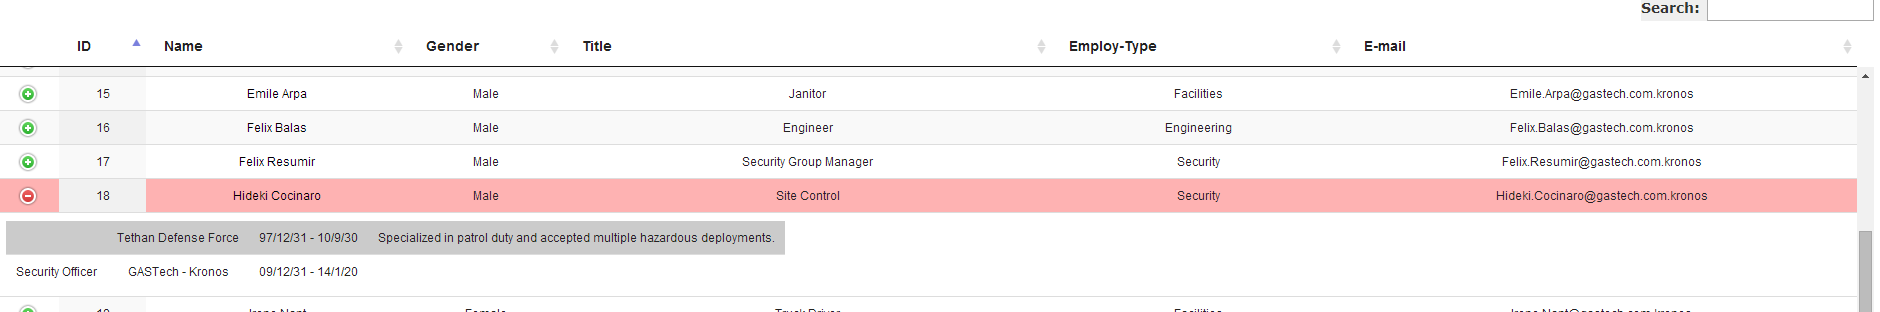
\includegraphics[width=3in]{SingleExperienceLine2.png}
  \caption{Identify conflicts and check it using detailed description}
\end{figure}

\subsection{News timeline}
News timeline is designed to provide a quick view for the users to grab the development of an event and then focus on certain points to analyze. 
\par
As the volume of news data is large, simply displaying news in a timeline may be imbalance and will result in a lot of overlapping in a short period of time. So semantic zooming is used in News Timeline, which makes it possible to provide a compact view in the timeline when the time range is long and provide news position precisely when the range is short.
\par
Aside rooming function, News Timeline provides visual set operation on timelines. Every time a user searches a keyword, a new timeline will be generated and displayed on the screen. As timeline operations are allowed for users, a user can do set operations between them to refine the result he/she finds. Draggable dialogs are also provided to refine the data: a user can pick up important news he/she finds and arranges them in the timeline by dragging to prepare for further investigation.
\begin{figure}[htb!]
  \centering
  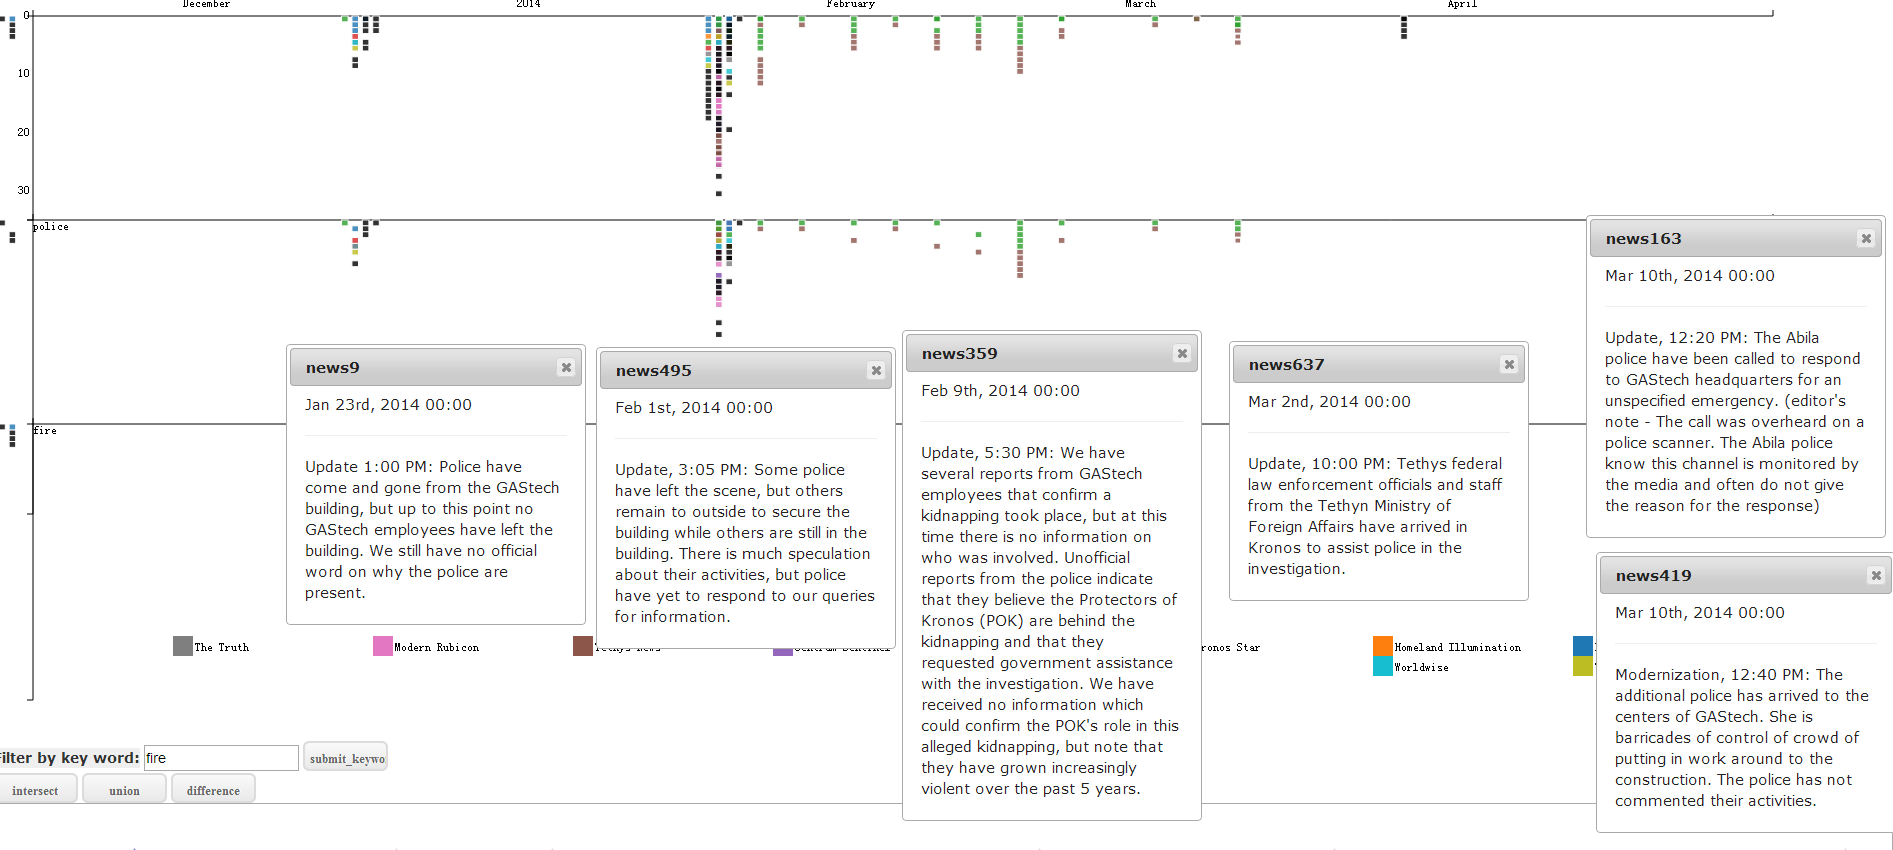
\includegraphics[width=3in]{image017.png}
  \caption{Using operational News-Timeline to pick up important events}
\end{figure}

\subsection{Email Reader}
\paragraph{Design And Overview}
In MC1 we have email headers from two weeks of internal GAStech company email, we can get a social network from this data and then discover communities. For MC1, we need to reveal the connections between GAStech employees and to find suspicious clues including the subject of emails. If there is an email containing words related to POK, then we can try to find the connections between the sender of the email's community and POK. Therefore we implemented a visual analytic tool for email headers based on D3.js. The tool is easy to use and effective to discover communities. 

\paragraph{Layout And User Interactions}
Our tool's layout containing four components, filters, email sending and receiving timeline, email headers view, and community view.
After selecting an employee through the filter, his/her email records will be depicted on the timeline, the contents of email headers will be put in the email headers view and some communities including him/her will be showed in the community view.  
\par
Users can interact with the layout both directly and indirectly, including selecting employees, filtering by keywords and limiting the size of groups. When a user consider a keyword or a person to be suspicious, he/she can easily see people who send the suspicious emails or are close to the suspicious person.
\begin{figure}[htb]
  \centering
  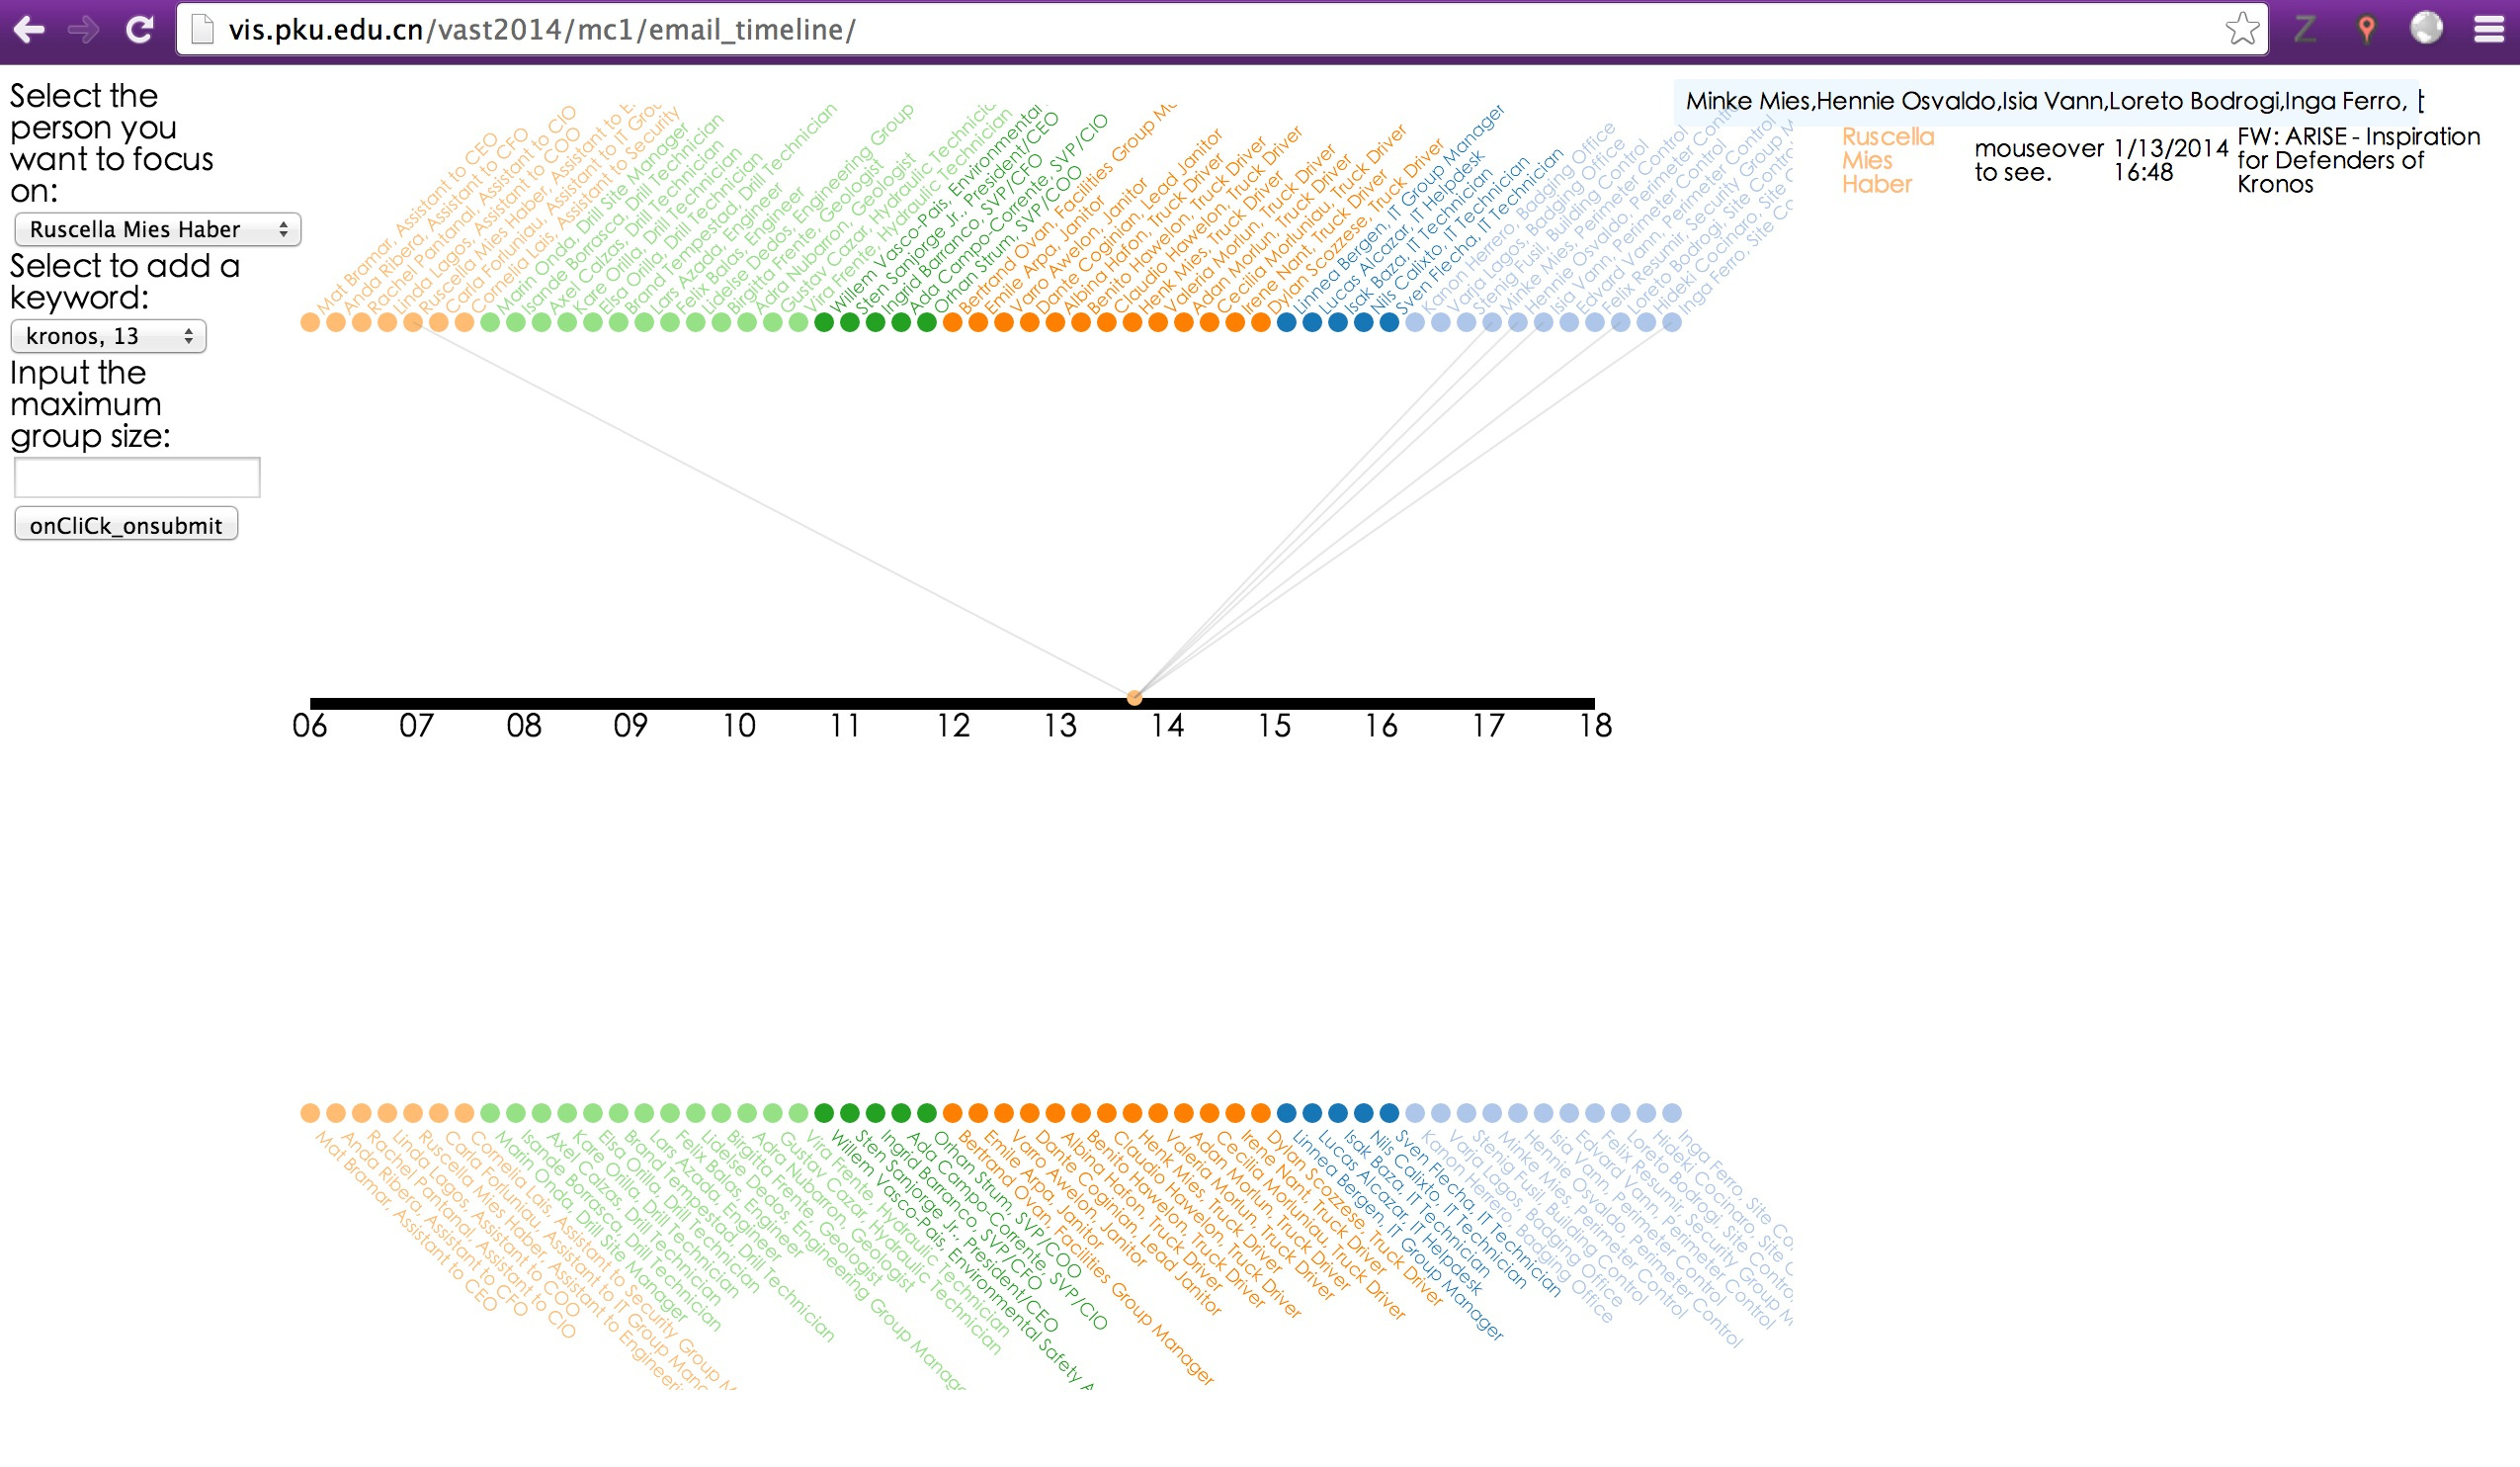
\includegraphics[width=3in]{image_et.png}
  \caption{Using Email Reader to identify the employee relationship}
\end{figure}

\section{Data Exploration}
In this section, we introduce how we use \projectname\ along with analysis tools like Jigsaw, Gephi to analysis MC1 data.
\par
As our tool only provides an overview of the whole data, we still need to use Jigsaw to assist the analysis process. And general analysis includes following steps:
\begin{enumerate}
\item Read report on POK and GAStech to identify important people involved in the conflicts.
\item With important entities identified, using News Timeline to pick up important events associate with them.
\item Cooperated with Jigsaw and Fusion to read news articles and find relationship between POK and GAStech.
\item Discover important communities and identify suspicious people through Resume Reader and Email Reader.
\item Display the result by putting important news in the timeline and draw the relationship network with Gephi.
\end{enumerate}
\par
With rounds of exploration, we are able to identify suspicious people and pick up events related to the employee missing events. Results are presented in forms of timeline events and relationship net work to provide for further investigation in Grand Challenge.

\section{Conclusion}
\projectname\ provides user the ability to extract important events from huge volume of news articles and the ability to analyze conflicting data of employee resume.
\par
 With the help of \projectname, we successfully identify a group of GAStech people who are suspicious to get involved in the kidnap event. Our visual analysis tools emphasize on analyzing text data from different sources and provide an overview of the whole dataset.
 \par
 Visualization tools to display results we found are also necessary and that can be part of future work.
%% if specified like this the section will be ommitted in review mode
\acknowledgements{
We have special thanks to Miss Dong Liu for her compiling raw materials to inspire our design on visualization tools.
}
\bibliographystyle{abbrv}
%%use following if all content of bibtex file should be shown
%\nocite{*}
\bibliography{template}
\end{document}
